% LLVM is a set of compiler and toolchain technologies that can be used to
% develop a front end for any programming language and a back end for any
% instruction set architecture. LLVM is designed around a language-independent
% intermediate representation (IR) that serves as a portable, high-level assembly
% language that can be optimized with a variety of transformations over multiple
% passes. The name LLVM originally stood for Low Level Virtual Machine, though
% the project has expanded and the name is no longer officially an acronym. 
\subsection{Инсталиране на Rust}
Rust е език, който използва LLVM за обръщането на код в машинни инструкции.
% TODO: какво е машинна инструкция
LLVM е набор от технологии за компилиране, които позволява да бъдат написани
различни frontend-ове за всеки език и backend-ове за всяка хардуерна архитектура.
Благодарение на този факт, Rust може да работи на всички модерни операционни системи
като Windows, MacOS, Linux, OpenBSD и още много други.

За операционните систтеми базирани на UNIX принципите, като MacOS и Linux можем
да инсталираме Rust с една проста команда:
\begin{lstlisting}
curl --proto '=https' --tlsv1.2 -sSf https://sh.rustup.rs | sh
\end{lstlisting}

Или през package manager-а на операционната система.
В MacOS можем да използваме Homebrew. За да инсталираме Rust, трябва да изпълним следните команди:
\begin{lstlisting}
/bin/bash -c "$(curl -fsSL https://raw.githubusercontent.com/Homebrew/install/HEAD/install.sh)"

brew install rust
\end{lstlisting}

Когато използваме Linux и искаме да инсталираме компилатора, трябва да се
съобразим с това каква дистрибуция използваме. Най-често използваните такива
са: \begin{itemize}
\item Arch Linux - pacman -S rustup
\item Debian Linux - apt-get install rustup
\item Fedora Linux - dnf install rust cargo
\end{itemize}

% TODO: mention WSL
За да инсталираме Rust на Windows, трябва да изтеглим 64 или 32 битовия
инсталационен файл от сайта на Rust: https://rustup.rs/. 

\begin{figure}[!htb]
  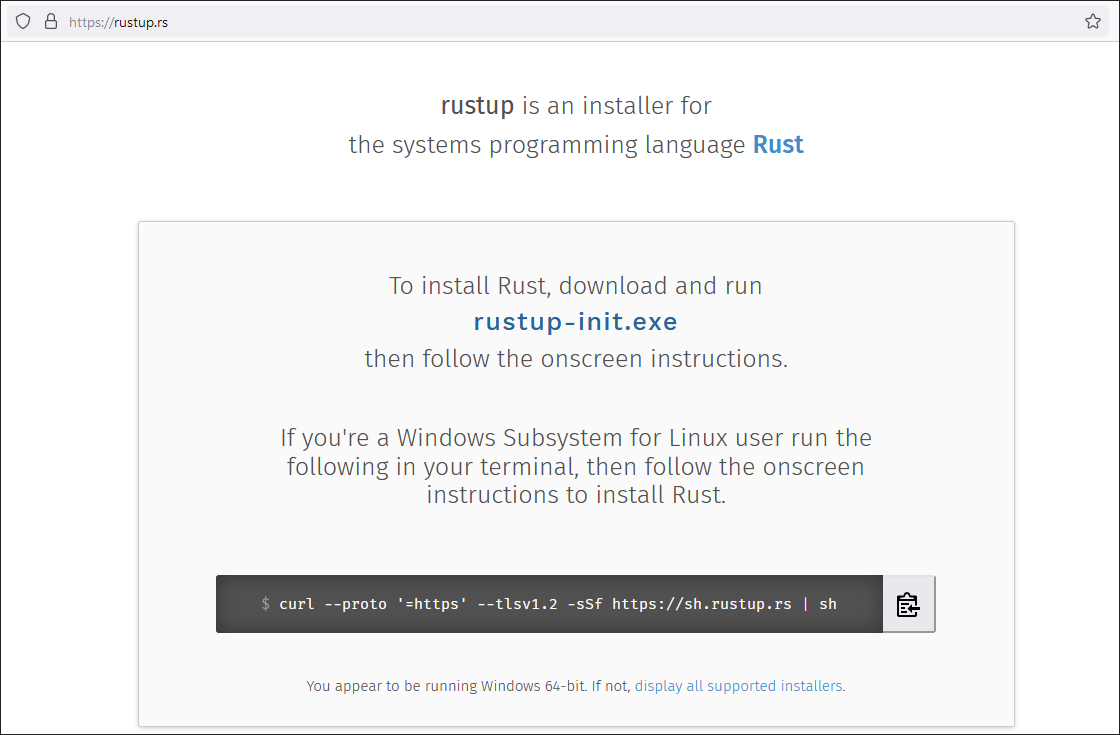
\includegraphics[scale=0.32]{rust-up-windows-install}
  \centering
  \caption{Сайт за изтегляне на инсталационния файл на Rust за Windows}
  \label{fig:rust-up-windows-install}
\end{figure}
